\chapter{Техническое задание}

Спроектировать и провести моделирование двухканальной приёмной ячейки с управляемым фазовым сдвигом в каналах и фильтрацией в соседних каналах.

Приёмная ячейка должна быть настроена на центральную частоту $F_c = 8.9~\text{ГГц}$ с полосой пропускания равной $F_{HPBW} = 530~\text{МГц}$.
Коэффициент усиления в полосе пропускания должен быть не менее, чем $K_p = 38~\text{дБ}$ с уровнем неравномерности, не превыщающим $3~\text{дБ}$.
Необходимо также обеспечить запирание не ниже $\Delta A_{stop} = 35~\text{дБ}$ в полосах частот $(7.7-8.2)~\text{ГГц}$ и $(9.6-10.1)~\text{ГГц}$.
Коэффициент шума не должен превышать значение $K_{ш} = 2.9~\text{дБ}$.
Использовать фазовращатель с шагом не более $12^\circ$.

Структурная схема проектируемого устройства представлена на Рис.~\ref{fig:tor_structure_schematic}.

\begin{figure}[!ht]
    \centering
    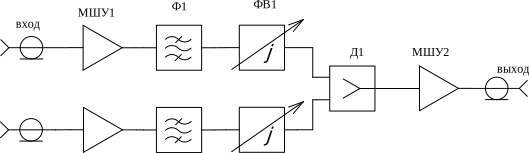
\includegraphics[width=\textwidth]{tor_structure_schematic.pdf}
    \caption{Структурная схема проектируемого устройства}%
    \label{fig:tor_structure_schematic}
\end{figure}

\begin{figure}[!ht]
    \centering
    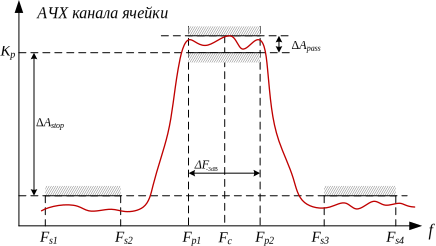
\includegraphics[width=\textwidth]{tor_response.pdf}
    \caption{Пояснение к ТЗ на АЧХ канала}%
    \label{fig:tor_response}
\end{figure}

Общие условия и пояснения:
\begin{enumerate}
    \item
        КСВН по всем ВЧ-входам и ВЧ-выходам должен быть не более $1.5$ в рабочей полосе частот.
    \item
        Фазовращатель должен быть аналоговым или дискретным с шагом фазы не более заданного.
        Полный диапазон перестройки должен быть в 360°.
    \item
        Предпочтительно чтобы первым устройством был фильтр Ф1, однако, если из-за потерь на фильтре Ф1 невозможно удовлетворить на Кш, то первый МШУ с минимальным коэффициентом шума можно поставить первым.
    \item
        Рабочий диапазон частот $F_{p1} \ldots F_{p2}$ определяется как размах $\Delta F_\text{-3~dB}$ относительно центральной частоты $F_c$, т.е. $F_{p1} = F_c - 0.5 \Delta F_\text{-3~dB}$ и $F_{p2} = F_c + 0.5 \Delta F_\text{-3~dB}$.
    \item
        При расчете $K_\text{ш}$ канала строить упрощённую модель (только в один канал, при задании свойств сумматора учитывать только омические потери, без потерь на деление).
\end{enumerate}
